%%% DOCUMENT SETUP %%%
\documentclass[11pt,a4paper,onecolumn]{article}
\usepackage[greek,english]{babel}

%%% LAYOUT %%%
\usepackage{fullpage}
\usepackage[parfill]{parskip}
\usepackage{multicol}
\usepackage{footnote}

%%% GRAPHICS %%%
\usepackage{graphicx}
\usepackage{color}
\usepackage{graphics}
\usepackage{rotating}
\usepackage{subfig}
\usepackage{amsmath}
\usepackage{amssymb}
\usepackage{amscd}
\usepackage{xfrac}
\usepackage{float}
\usepackage{dsfont}

%%% FONT %%%
\usepackage{ifxetex}
\ifxetex
  \usepackage{fontspec}
    \setmainfont{Linux Libertine O}
  \usepackage{xunicode}
  \usepackage{microtype}
\else
  \usepackage[T1]{fontenc}
  \usepackage[latin1]{inputenc}
  \usepackage{times}
  \usepackage{microtype}
\fi

%%% Coding %%%
\usepackage{listings}
\usepackage{algorithm}

%%% TITLE PAGE %%%
\author{Jeroen Hofman (10194754)  \\
  Grid Computing: Computational Science \\
  [15pt] University of Amsterdam (\textsc{UvA})}

\title{Modeling Civil Violence\\
		}

\begin{document}
\maketitle
\captionsetup{width=0.8\textwidth}
\graphicspath{{/home/jhofman/Desktop/2c2012/CSS/Figures/}}
\thispagestyle{empty}

%%% ABSTRACT %%%
\begin{center}
\begin{abstract}
\small{I implemented a model of civil violence on a 2D grid as proposed by Epstein. I made modifications to this model; a parameter sweep on the vision range and the implementation of different movement strategies. A parameter sweep on the vision range revealed a big difference in behavior, from constant levels of activity at small vision range to total suppression of activation at high vision range. Vision range values from 5-7 produce interesting behavior where the amount of activity spikes at intervals of random length. Implementing different movement strategies produces results as expected, the combination of movement strategies produces interesting results due to positive feedback loops.}
\end{abstract}
\end{center}

%%% TABLE OF CONTENTS %%%
\newpage
\tableofcontents
\newpage

\section{Introduction}
In this report we are investigating the modeling of civil violence with an agent-based model.I extended the work of Epstein \cite{Epstein}, which has done fundamental work in this area. Recently Clemens et al. \cite{Epstein2} has provided some evidence for the validity of the model as constructed by Epstein. More specifically, assumptions Epstein makes about hardship and legitimacy of a regime seem to be consistent with empirical observations. Many extensions on Epstein's model have been made, including a project by the American military called MANA, using specific agent-based models for strategic implementations. Indeed, much research has been done in making the agents more clever, let them exhibit strategies and let them evolve, see for instance \cite{Quek}.

In this report we will investigate two different aspects of Epstein's original model:
\begin{itemize}
\item
  What is the effect of the agents vision range on outbursts of rebellion during the simulation as reported by Epstein?
\item
  What is the effect of small improvements in movement strategies as opposed to Epstein's random movement?
\end{itemize}

\section{Model}
We will describe an agent-based model of civil violence on a 2D grid based on a paper by Epstein \cite{Epstein}. We assume two kinds of agents, civilians and cops. The cops are loyal to an unspecified regime. In the following paragraphs we will introduce many variables, a motivation on the significance of parameters and their values can be found in Epstein's paper. We will focus on a few variables which we will investigate further. We will first quickly repeat the agent dynamics as implemented by Epstein.

\subsection{Agent Rules}
We first specify the civilian dynamics. Every civilian has two properties defining its grievance against the regime, called hardship $H$ and legitimacy $L$. Hardship is a measure for the amount of 'suffering' each civilian has to endure. The value for each civilian is drawn randomly between 0 and 1. The legitimacy of the regime is set by a constant value which is the same for each civilian, assuming all civilians experience equal pressure from a central authority. The grievance $G$ of each civilian against the regime is then given by:

\begin{equation}
  G = H(1 - L)
\end{equation}

i.e. if the legitimacy of a government is unchallenged, the grievance will be 0, the same holds for a hardship level of 0. We can further introduce some kind of heterogeneity among the civilians, namely their appetite for taking risk, defined by the level of risk aversion $R$, randomly drawn between 0 and 1 for every agent.

Every civilian has the choice between two states, being inactive or active (rebelling). A civilian decides on its state by looking at its environment, defined by its vision range $v$, which is a square block of size $2v + 1$ with the position of the civilian as its center. Within this vision range a ratio of cops versus active civilians is computed and an arrest probability is defined as:

\begin{equation}
  \label{eq:arrestprob}
  P = 1 - \exp( - k \lfloor(C/A)_v\rfloor)
\end{equation}

where $k$ is chosen such that in the case of a ratio of 1 the arrest probability as estimated by the civilian is set to 0.9, giving $k = 2.3$. Hence the more civilians are active, the lower the arrest probability. This makes sense because of the cop dynamics which will be explained later. The flooring of the ratio is important although Epstein does not mention it in his paper. A Net-logo implementation of this model also uses flooring, since any interesting behavior completely disappears without it (the same holds for the model described in this report). Every civilian has a net risk defined by $N = RP$ according to the above formulas. The following rule is now applied for determining the state of an agent:

\begin{equation}
\text{state} =
\left\{
    \begin{array}{rcl}
      \text{active} & \mbox{if} & $G - N > T$\\
      \text{inactive} & \mbox{otherwise} &
    \end{array}
\right.
\end{equation}

where $T = 0.1$ is the global threshold. This concludes the civilian description.

The cop rules are much simpler, it has a vision range as well, which for simplicity we will take equal to the civilians vision range $v$. A cop will look at all the active civilians in its vision range and arrest one. The cop will move to the agents position and the agent will be jailed, hence unable to do anything, for a random jail term picked uniformly between 1 and $maxJail$.

\subsection{Algorithm}
Using the agent rules as described above, we can now set up an algorithm. Given a density of civilians $\rho_{\text{civ}}$ and a density of cops $\rho_{\text{cop}}$ we place them randomly on a 2D grid of size 40x40, with continuous boundary conditions on all sides, effectively bending the rectangular grid in a torus. Every civilian obtains a grievance level and a risk aversion according to the rules described above.

Every iteration of the algorithm we create a shuffled list consisting of all the agents together (so civilians and cops). We then go through this list one by one. When an agent is selected, it first applies a movement rule; it moves to a random unoccupied location in its vision range. If the agent is a civilian and not jailed, it then proceeds by computing $P$ according to equation \ref{eq:arrestprob} and it uses the threshold $T$ to determine its state. If the agent is a cop, it looks for active civilians within its vision range, selects one randomly and sends it to jail. The cop also moves to the position of the arrested agents. Arrested civilians are skipped in the algorithm since they cannot do anything. Although arrested civilians stay on the grid, their position can be occupied by non-jailed civilians or cops.

We run the model for a number of iterations $maxIter$. Every iteration the number of active, inactive and jailed civilians is computed. The number of cops is constant throughout the whole simulation.

Since the number of free parameters in this model is large, we fix a number of parameters, using the values from Epstein's paper or values close to his values. We fix the following parameters:

\begin{table}[H]
  \centering
  \begin{tabular}{l | l}
    Parameter & Value \\
    \hline
    $N$ & 40 \\
    $\rho_{\text{civ}}$ & 0.70 \\
    $\rho_{\text{cop}} $ & 0.04 \\
    $L$ & 0.8 \\
    $T$ & 0.1 \\
    $maxJail$ & 15 \\
    $k$ & 2.3 \\
  \end{tabular}
  \caption{Fixed parameters.}
  \label{tab:param}
\end{table}

\subsection{Modifications}
The model and algorithm as described above are taken from Epstein's paper. Two different types of adjustments are added to the model to test certain hypotheses as mentioned in the introduction.

Firstly we want to investigate the outburst behavior using different values of the vision range. The vision range is the same for the civilians and the cops. Epstein used a value of 7 as the default vision range. We tested vision range values between 3 and 9 to investigate the effect of the vision range on the outcome of the model.

A second modification we implemented is the movement of the agents. We implement different movement strategies, both for the civilians and the cops. These modifications are the following:

\begin{itemize}
\item
  Civilian: If the civilian is active, it will try to seek a safe place instead of randomly moving to an unoccupied point in its vision range. To implement this, an active civilian moves to an unoccupied random spot in the quadrant of its vision range which contains the most active civilians. Hence active civilians exhibit some kind of herding, i.e. the active civilians will tend to move towards each other, hopefully giving a smaller probability of getting arrested. If no active civilians are present except itself, it moves randomly. Inactive civilians also move randomly, as before. We expect this strategy to be beneficial for the active agents.
\item
  Cop: Instead of randomly moving and then arresting an active agent it has the opportunity to directly arrest an agent. If no active civilians are in sight, it moves randomly and then tries to arrest one (if any are present), as before. We expect this strategy to be beneficial for the cops.
\end{itemize}

We will implement these changes in the model and investigate the effect of these relatively simple changes.

\section{Results}
First we look at the general behavior of Epstein's model. We performed a simulation consisting of $10^5$ iterations with a vision range of 6. The other parameters are given by table \ref{tab:param}. We use the original random movements as described by Epstein. Figure \ref{fig:sample} below shows the location of agents on the grid, in which green dots are inactive civilians, red dots are active civilians, black dots are cops and blue dots are jailed civilians. We can distinguish roughly three types of macroscopic states of the system: A quiet state in which most civilians are inactive (left), an active state in which a significant part of the civilians is active (middle) and an jailed state in which a significant portion of the civilians is jailed (right).

\begin{figure}[H]
  \centering
  \subfloat{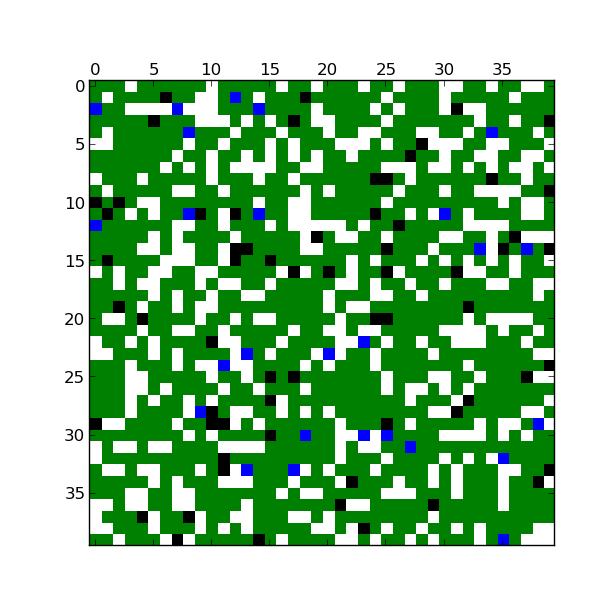
\includegraphics[width=0.33\textwidth]{state_1.png}}
  \subfloat{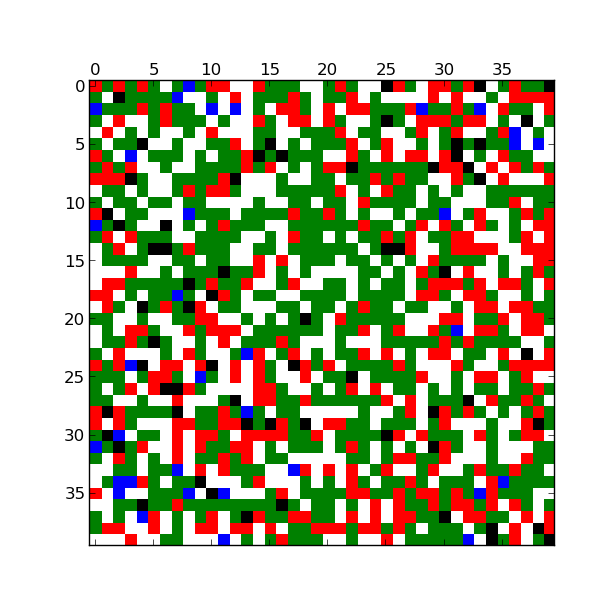
\includegraphics[width=0.33\textwidth]{state_2.png}}
  \subfloat{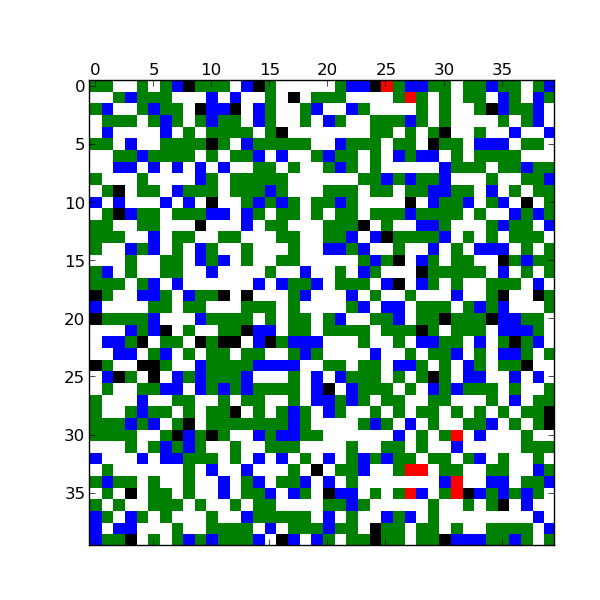
\includegraphics[width=0.33\textwidth]{state_3.png}}
  \caption{Three possible states: inactive state (left), active state (middle), jailed state (right).}
  \label{fig:sample}
\end{figure}

The behavior of the model in terms of the number of agents with a certain state is given in figure \ref{fig:6} below. The horizontal axis is the time axis, in this case equal to the number of iterations. Clearly there are very sharp outbursts of active civilians, in between outbursts the number of active civilians is nearly zero. Right after an outburst the number of jailed agents peaks, this then declines but is always at some nonzero number, caused by a few civilians becoming active every turn but arrested straight away. It is interesting to see that all the outbursts have a similar peak height, namely around 400. This number is specific for the parameter set used here, it is a maximum caused by the number of civilians able to become active (due to personal grievance levels), the density of cops on the grid and the fact that at some point the active civilian level is so high that all cops (64 in number) arrest an active civilian every iteration. This causes local active civilian density to drop and so the more risk-aware civilians will return to their quiet state, causing a chain reaction which ends the outburst.

\begin{figure}[H]
  \centering
  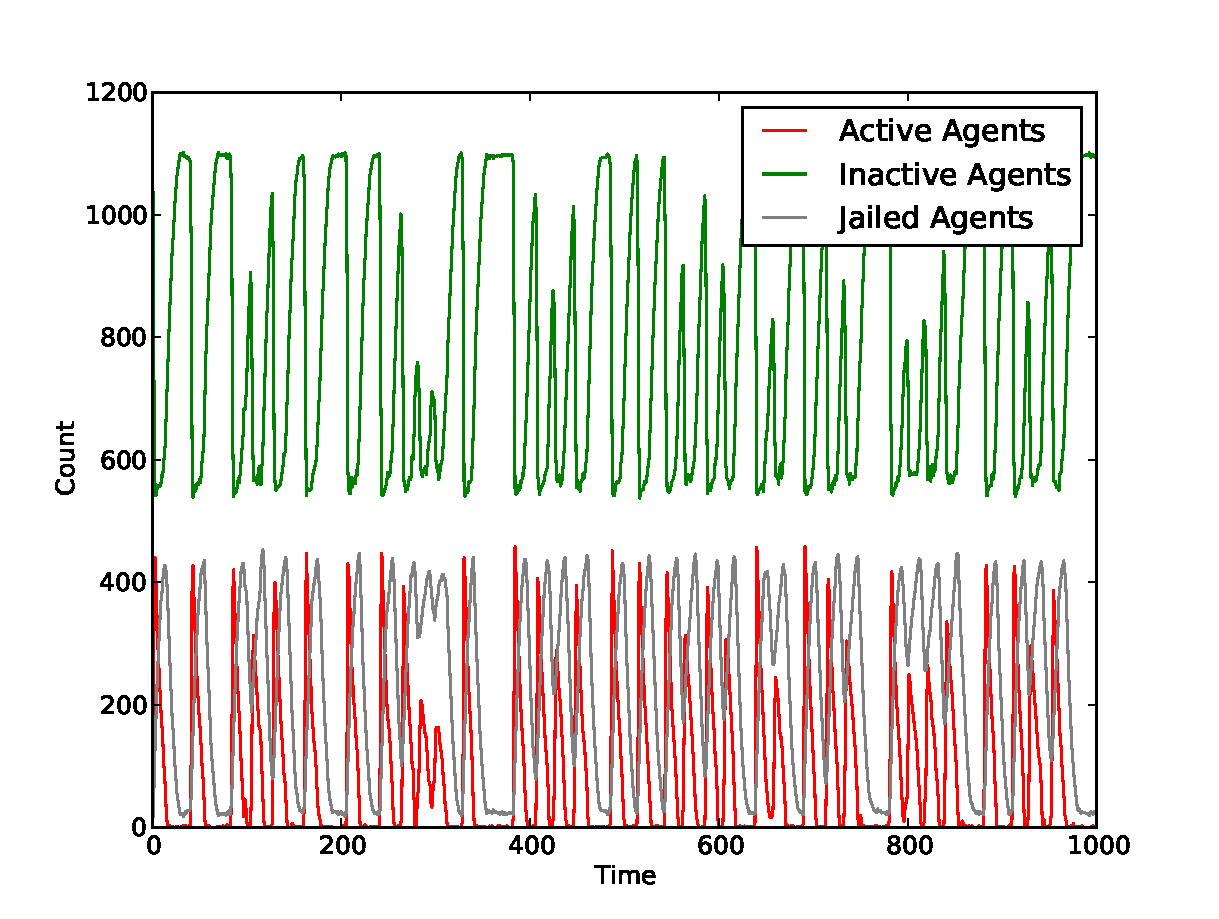
\includegraphics[width=0.7\textwidth]{original_sample.pdf}
  \caption{Time-series of the number of agents.}
  \label{fig:6}
\end{figure}

\subsection{Vision Range}
We will now analyze the results for different vision ranges from 3 up to 9. We performed a simulation over $10^5$ iterations for vision ranges of 3, 5, 6, 7 and 9. We will first investigate the 'extreme' values, i.e. 3 and 9. In the case of a vision range of 3, we obtain results as shown in figure \ref{fig:3} below. It is clear from the figure that the outburst behavior has completely disappeared. Instead, the number of agents in each state fluctuates with small margins around a certain equilibrium values which is reached very early in the simulation. The reason for this behavior is two-fold, due to the small vision range small regions of high activity do not perturb through the grid before they are killed by cops sending the agents to jail. On the other hand, also due to the small vision range, cops are not able to effectively kill any activity causing a constant number of active civilians to be present.

We also checked that the behavior we observe in figure \ref{fig:3} is characteristic behavior and not just incidental (depending on the random distribution of grievance or the random initial placement of agents for instance). Therefore we simulated, with a vision range of 3, 1000 iterations 1000 times with a random initial startup. We compute an average activity of 99.68 $\pm$ 0.62 (standard deviation), so all te measurements are very close to another, showing that the behavior of figure \ref{fig:3} is representative. Due to long simulation times we assume but will not show that all following measurements are representative measurements for the given parameters. Hence we for instance assume that information about the initial condition will be lost after a sufficient amount of time, such that the number of outbursts does not depend on specific initial conditions and is the same for each run.

\begin{figure}[H]
  \centering
  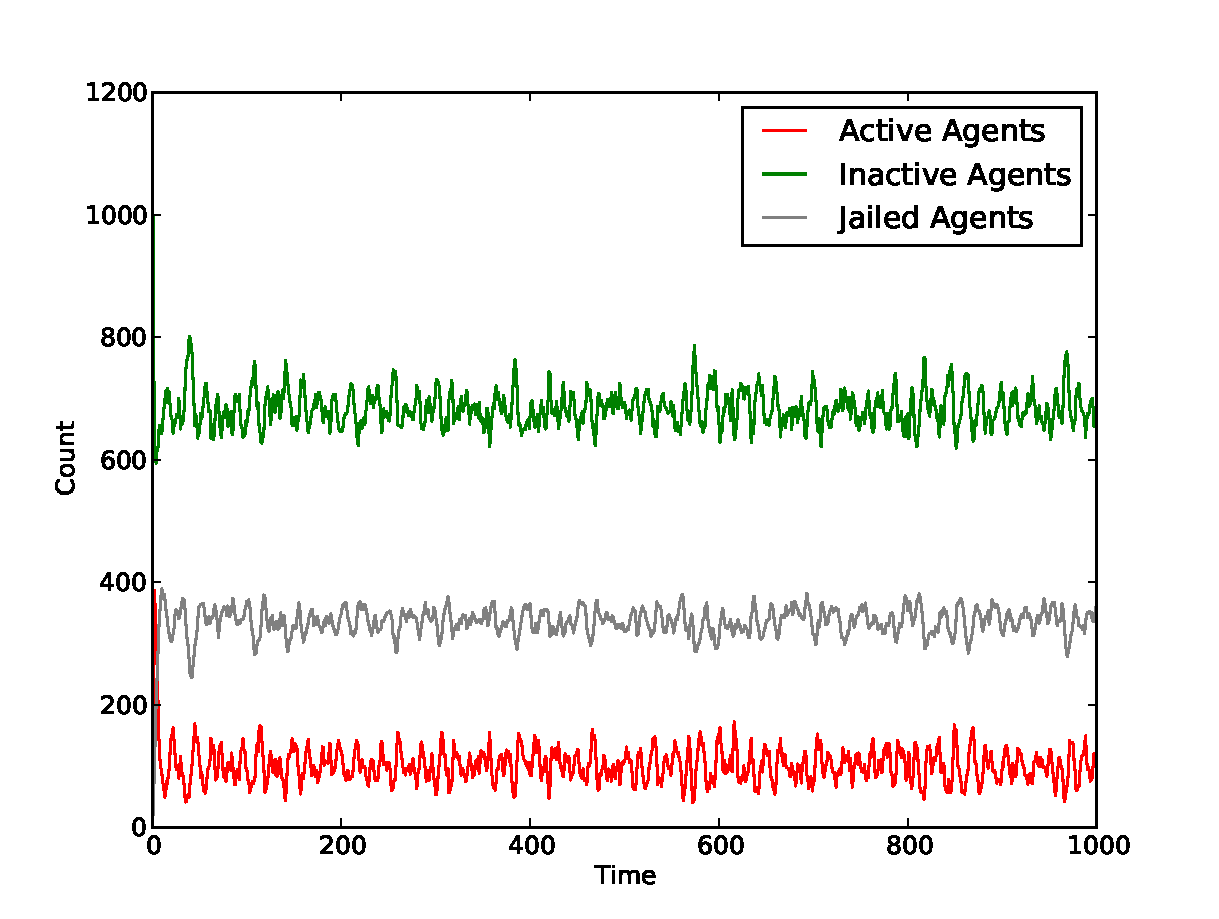
\includegraphics[width=0.7\textwidth]{original_3.pdf}
  \caption{Time-series of the number of agents.}
  \label{fig:3}
\end{figure}

If we set the vision range to 9, all outburst behavior is again suppressed, but the activity is always 0 or close to 0. This is caused by the cops being able to survey large areas (almost a quarter of the grid with a vision range of 9) and so effectively suppress any active civilians. Over the total of $10^5$ not one outburst occurred, making large vision ranges uninteresting.

We can look at the more interesting 'middle' cases, in particular we look at vision ranges 5, 6 and 7. We performed the same simulation as before and we counted the number of outbursts during $10^5$ iterations, where we specify an outburst to be a period with an activity count larger than 50. The results are given in table \ref{tab:outburst} below:

\begin{table}[H]
  \centering
  \begin{tabular}{l | l}
    Vision Range & Number of outbursts \\
    \hline
    5 & 5316 \\
    6 & 2935 \\
    7 & 376
  \end{tabular}
  \caption{Number of outbursts per vision range.}
  \label{tab:outburst}
\end{table}

Clearly when the vision range increases, the number of outbursts decreases, this is due to increased level of control by the cops, for which it is easier to immediately kill any active civilians. In this sense the simulation with the vision range of 3 as discussed above can be seen as one continuous outburst. We can also see this difference in frequency of outbursts clearly from a time-series, see figure \ref{fig:originals} below. Notice that the maximum number of active civilians is the same for different vision ranges, suggesting that this has no influence on the maximum.

\begin{figure}[H]
  \centering
  \subfloat{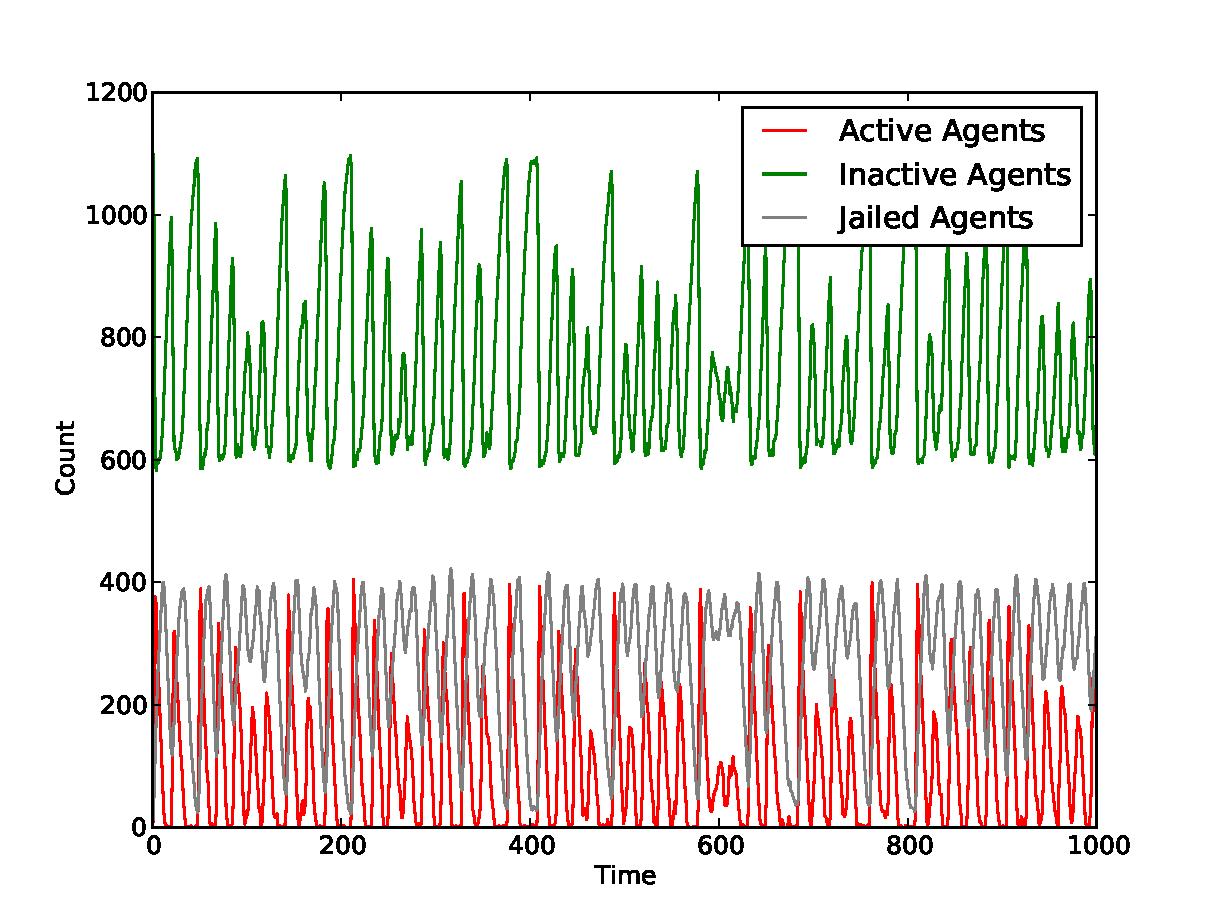
\includegraphics[width=0.33\textwidth]{original_5.pdf}}
  \subfloat{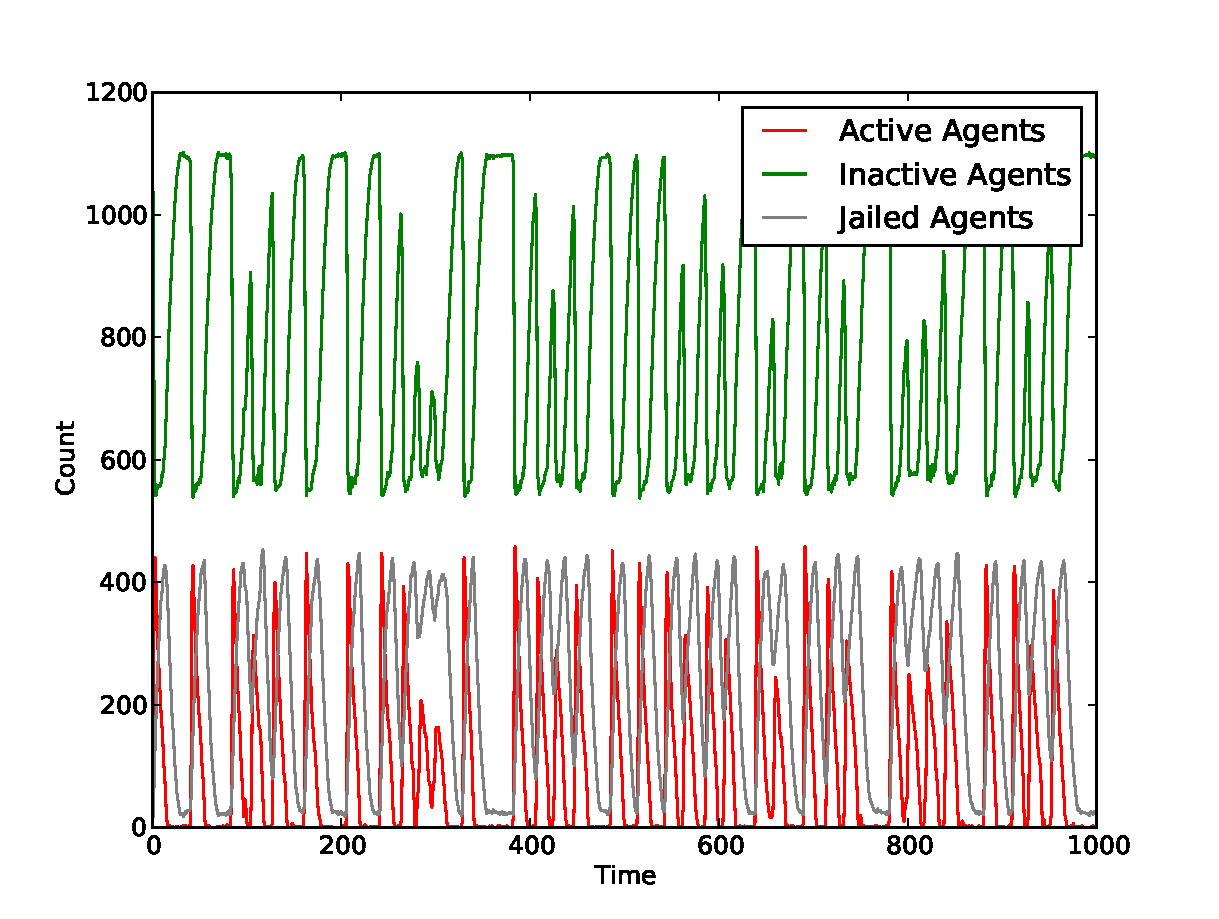
\includegraphics[width=0.33\textwidth]{original_sample.pdf}}
  \subfloat{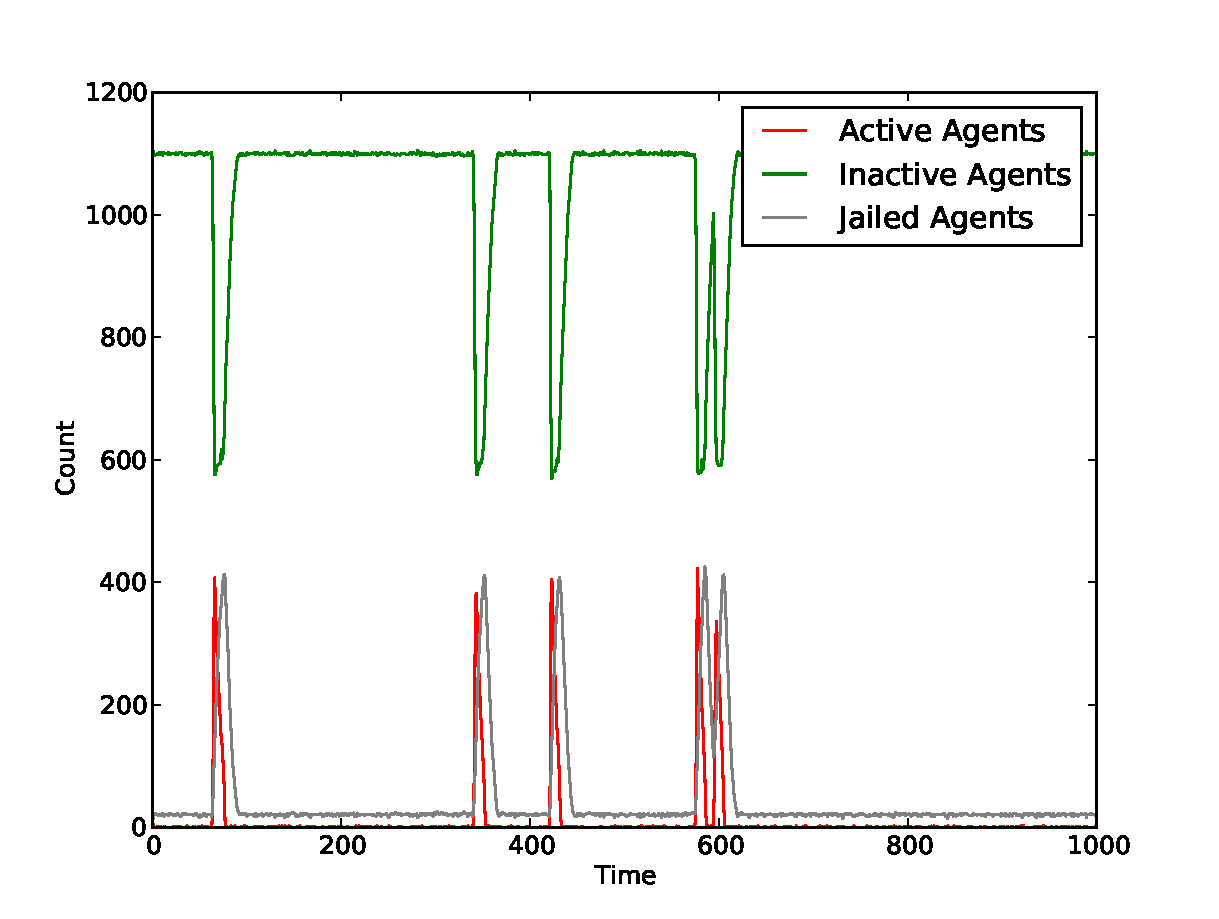
\includegraphics[width=0.33\textwidth]{original_7.pdf}}
  \caption{Time-series for vision ranges of 5 (left), 6 (middle) and 7 (right).}
  \label{fig:originals}
\end{figure}

\subsection{Movement Strategies}
In the second part we will investigate the effect of different movement strategies. For clarity we will distinguish four strategies:

\begin{itemize}
\item
  Strategy I: The original random movements as implemented by Epstein.
\item
  Strategy II: Active civilians move to the most 'active' quadrant, see section 2.3.
\item
  Strategy III: Cops can directly arrest an active civilian, see section 2.3.
\item
  Strategy IV: Strategy II + Strategy III
\end{itemize}

We performed a simulation of all four strategys with $10^5$ iterations and a vision range of 6 which, in the original model, gives bursting behavior. In order to analyze more in-depth we employ extra statistics next to the time-series as used in the sections above. We look at three different distributions generated from the data available for the simulation. Figure \ref{fig:dist} shows these distributions for strategy I. The upper left distribution is the waiting time distribution, giving the time between the end of an outburst and the start of the next. Outburst is again defined as an activity level above 50. The lower left distribution is the total activation distribution, which is the discretized integral over an outburst period. The right distribution is the outburst duration, i.e. the number of iterations there was an outburst. Figure \ref{fig:dist} resembles qualitatively the results obtained by Epstein which are shown in figure \ref{fig:Epstein}. The distributions follow the same shape.

\begin{figure}[H]
  \centering
  \subfloat{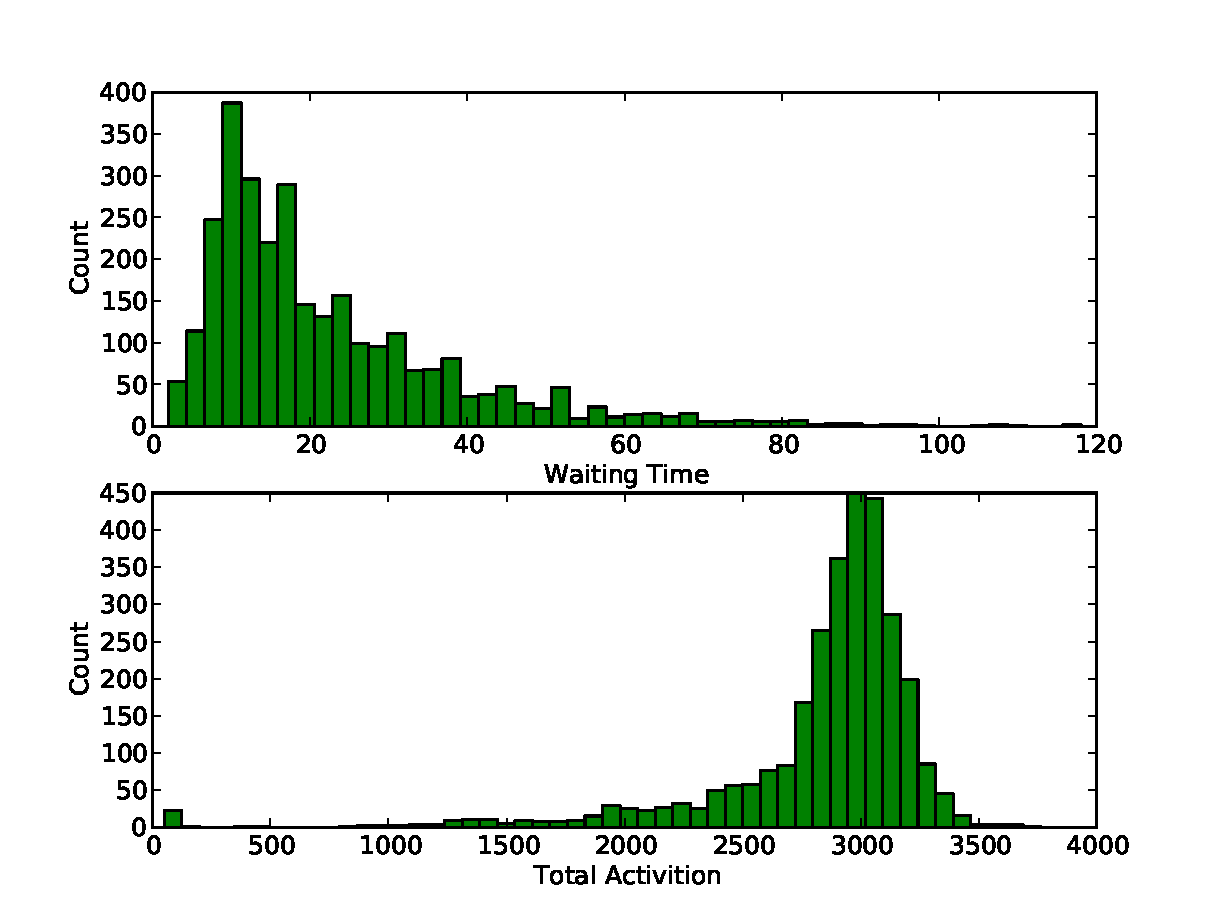
\includegraphics[width=0.5\textwidth]{original_dist.pdf}}
  \subfloat{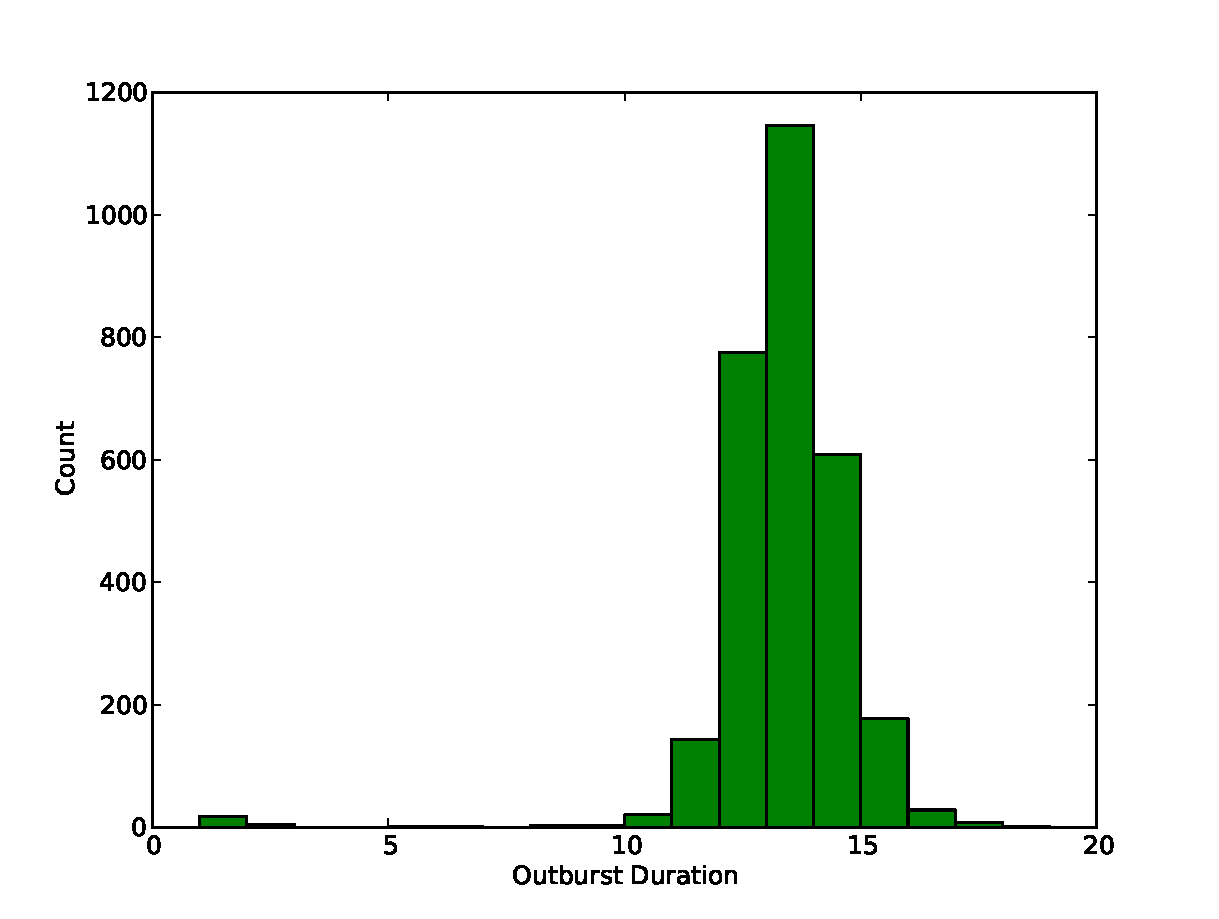
\includegraphics[width=0.5\textwidth]{original_outburst.pdf}}
  \caption{Waiting time distribution (top left), total activation distribution (bottom left) and outburst duration (right) for a vision range of 6.}
  \label{fig:dist}
\end{figure}


\begin{figure}[H]
  \centering
  \subfloat{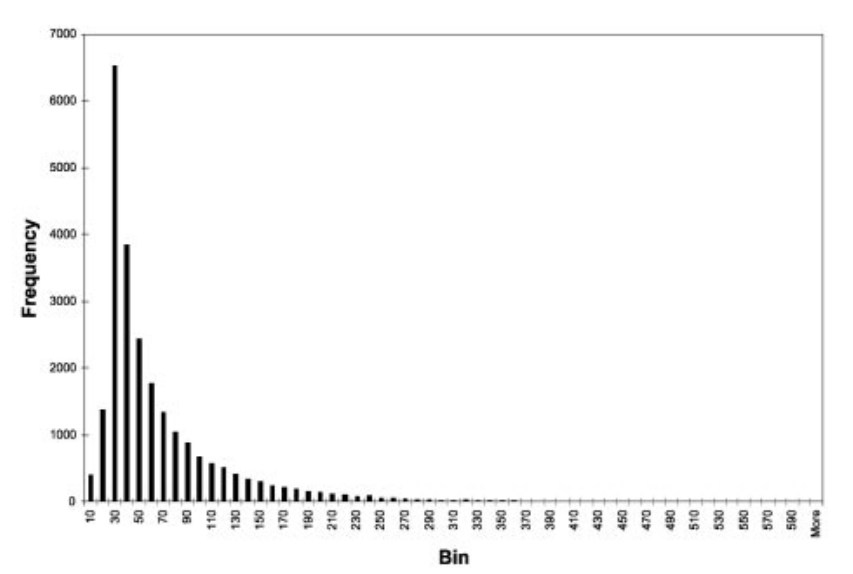
\includegraphics[width=0.5\textwidth]{Epstein1.png}}
  \subfloat{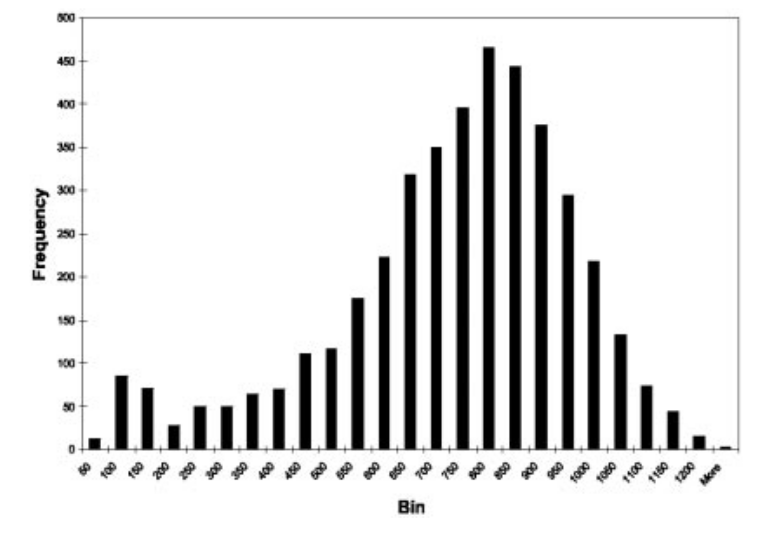
\includegraphics[width=0.5\textwidth]{Epstein2.png}}
  \caption{Waiting time distribution (left) and total activation distribution (right) from reference \cite{Epstein}. The specific parameter settings are unknown.}
  \label{fig:Epstein}
\end{figure}

The waiting time distribution and the total activation distribution are clearly not normally distributed, but seem to be log-normally distributed. The outburst duration does seem to be normally distributed, but with some extra values added to the '1' bin, because of small outbursts which are immediately suppressed. In order to compare between the four different strategys as mentioned above, we look at median values of these distributions (the mean is less useful because of the skewness of the distributions and/or outliers) and at the number of outbursts as we did before. The results for the four strategys are given in table \ref{tab:results} below.

\begin{table}[H]
  \centering
  \begin{tabular}{c | c | c | c | c}
    Strategy & \# Outbursts & Median Waiting Time & Median Total Activation & Median Outburst Duration \\
    \hline
    I & 2935 & 17 & 2958 & 13 \\
    II & 3256 & 14 & 2559 & 12 \\
    III & 2629 & 30 & 2543 & 11 \\
    IV & 2057 & 30 & 1933 & 10
  \end{tabular}
  \caption{Measurements for the four strategys.}
  \label{tab:results}
\end{table}

If we restrict ourselves first by only looking at strategys I, II and III, we see that implementing more efficient active civilians produces an increase in the number of outbursts (strategy II), while the number of outbursts decreases when implementing more efficient cops (strategy III). This is also reflected in the waiting time, it reduces for strategy II and increases for strategy III. The difference in the medians of 14, 17 and 30 is significant by the Mann-Whitney U test (see \cite{Mann}). The total activation decreases for both strategys, which is unexpected for strategy II. This can be explained by looking at the distributions according to strategy II shown in figure \ref{fig:strategy2}. The tails to the left are much thicker than in strategy I (figure \ref{fig:dist}) so the increased amount in outbursts of strategy II relative to strategy I are caused by relatively small outbursts, hence decreasing the total activation. This is also reflected in the outburst duration which also decreases in strategy II relative to strategy I, also caused by small outbursts being added in strategy II. Strategy III behaves as expected, the total activation declines and the outburst duration declines as well.

\begin{figure}[H]
  \centering
  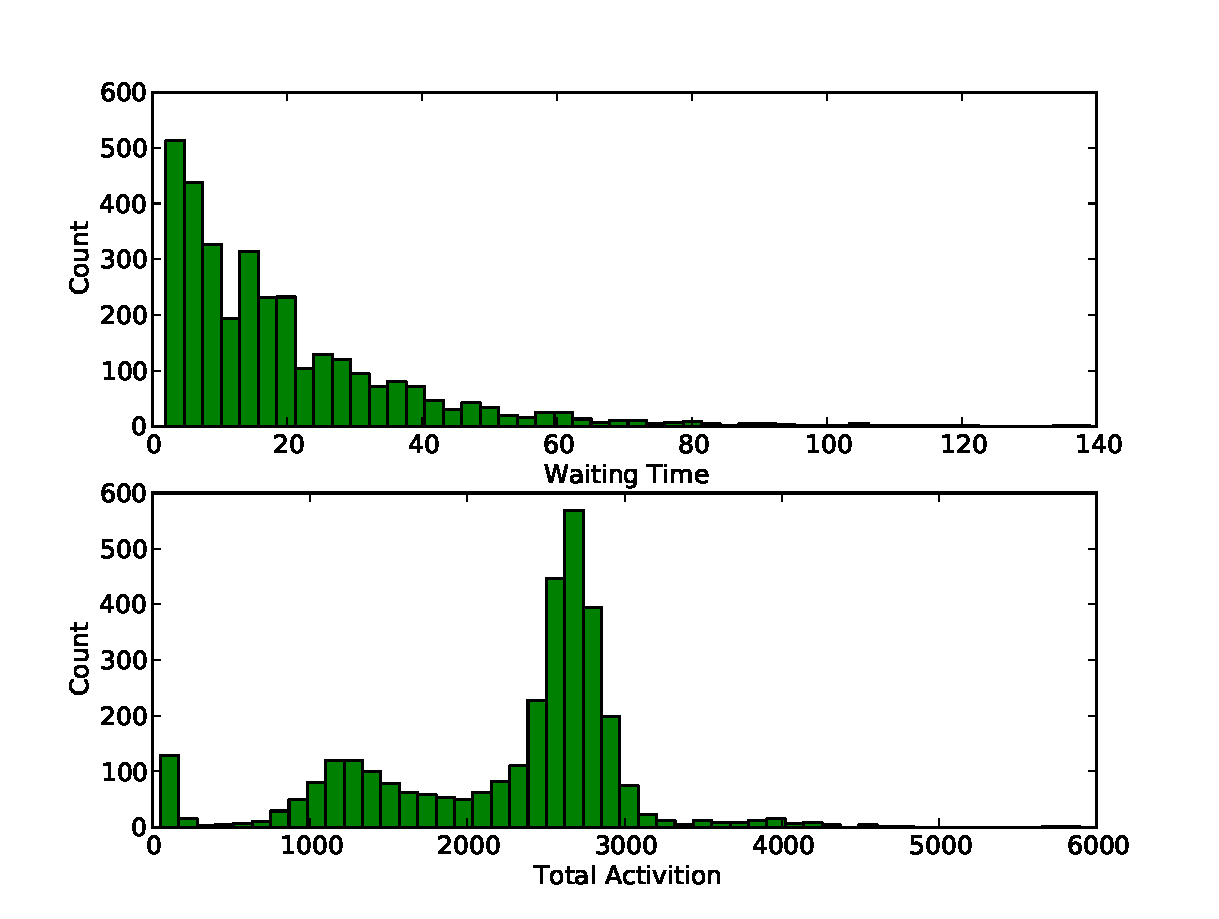
\includegraphics[width=0.7\textwidth]{moda_dist.pdf}
  \caption{Waiting time  and total activation distribution for strategy II.}
  \label{fig:strategy2}
\end{figure}

Strategy IV is a combination of both methods. The number of outbursts is greatly reduced, while the waiting time is the same as in strategy III. Also the total activation and the outburst duration are reduced. A possible explanation is that the herding introduced with strategy II actually helps the cops when they follow strategy III. Since they move efficiently and can stay at spots of high civilian activity (due to the movement rule of strategy III) they can quickly jail the active civilians there, while other active civilians also move to this same spot due to the still relatively high density of actives there. So in a sense the active civilians are lured by high concentration of actives, but quickly see that area taken over by cops, sending them to jail or force them to being inactive. It is interesting to see that the alternative movement strategies are working when they are implemented separately, but they positively reinforce each together from the cop perspective when implemented together.

\section{Conclusion}
We implemented a model of civil violence on a 2D grid as proposed by Epstein. We made modifications to this model; a parameter sweep on the vision range and the implementation of different movement strategies. A parameter sweep on the vision range revealed a big difference in behavior, from constant levels of activity at small vision range to total suppression of activation at high vision range. Vision range values from 5-7 produce interesting behavior where the amount of activity spikes at intervals of random length.
Implementing strategy II and strategy III give expected results. Strategy II give results which enhance civilian activity while strategy III suppresses that activity. A combination of the two in strategy IV led to a positive reinforcement of strategy III due to the clustering of active agents.

\newpage

%%% BIBLIOGRAPHY %%%
\begin{thebibliography}{7}
\bibitem{Epstein}
  J.M. Epstein, \emph{Modeling Civil Violence: An Agent-based Computational Approach.}, 2002, PNAS, Vol. 99, No. 3, 7243-7250
\bibitem{Quek}
  H. Queck, \emph{Evolutionary Game Theoretic Approach for Modeling Civil Violence.}, 2009, Evolutionary Computation, Vol. 13, No. 4, 780-800
\bibitem{Epstein2}
  B. Klemens et al., \emph{Empirical Performance of a Decentralized Civil Violence Model.}, 2010, Center on Social and Economics Dynamics Working Paper No. 56
\bibitem{Mann}
  H.B. Mann, D.R. Whitney \emph{On a Test of Whether one of Two Random Variables is Stochastically Larger than the Other.}, 1947, Annals of Mathematical Statistics, Vol. 18 No. 1, 50–60
\end{thebibliography}

\end{document}
